\documentclass{article}

\usepackage[utf8]{inputenc}
\usepackage[dvipsnames]{xcolor}
\usepackage{lmodern}
\usepackage{graphicx}
\usepackage{longtable}
\usepackage{tabularx}
\graphicspath{ {./images/} }
\usepackage{imakeidx}
\makeindex[columns=3, title=Alphabetical Index, intoc]

\usepackage{tabularx}
\usepackage{amsmath}
\usepackage{paralist}
\usepackage{enumitem}
\usepackage{hyperref} %\usepackage[hidelinks]{hyperref} %per togliere bordi rossi
\usepackage{makecell}
\usepackage{caption}
\usepackage[maxfloats=256]{morefloats}
\maxdeadcycles=1000

\usepackage[official]{eurosym}
\DeclareUnicodeCharacter{20AC}{\euro{}}

\author{Agosta, Belli, Emili, Giacchini, Luciani}

\begin{document}

\begin{center}
    \sffamily{\fontsize{50}{48} \selectfont \textcolor{red}{Nexi}\textcolor{green}{Fy}}
\end{center}

\begin{center}
    \itshape{\fontsize{20}{48} \selectfont streaming to your pocket}
\end{center}

\bigskip\bigskip\bigskip

\begin{flushleft}
    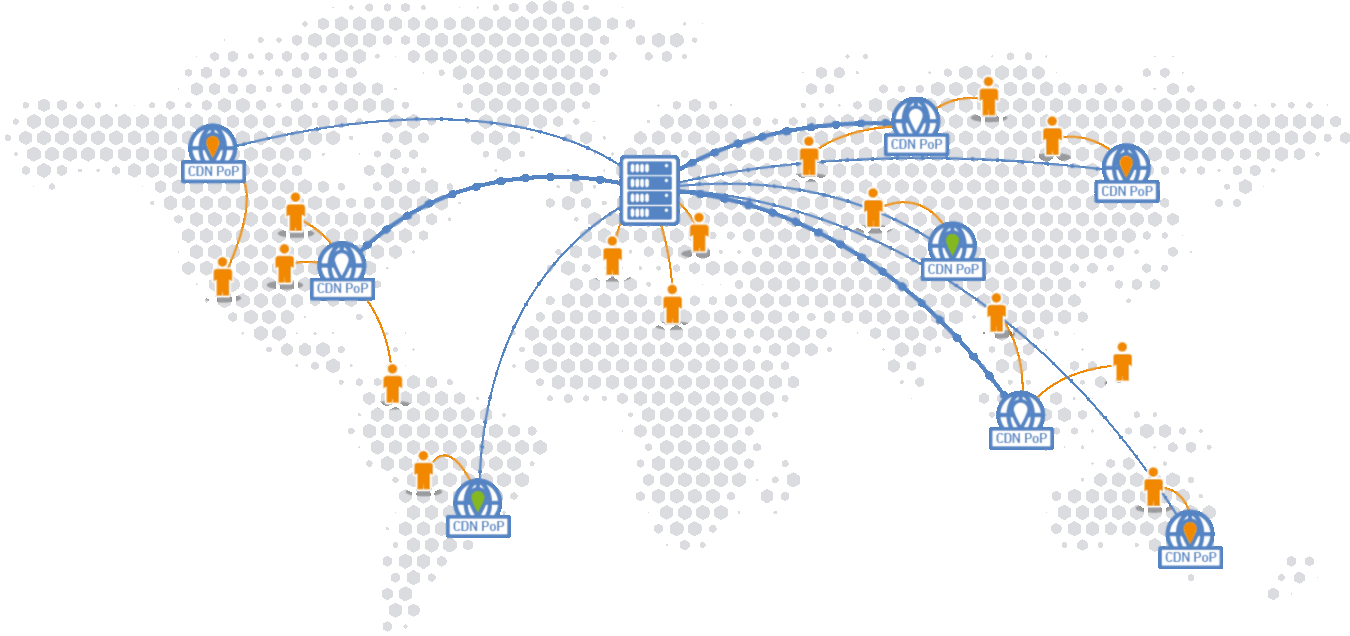
\includegraphics[scale=1]{../images/worldCDN.png}
\end{flushleft}

\bigskip\bigskip\bigskip

\begin{center}
    \itshape{\fontsize{30}{48} \selectfont Analisi dei Requisiti}
\end{center}

\newpage
\printindex

\newpage
\section{\itshape{Analisi dei Requisiti}}


\subsection{Requisiti Funzionali}
\begin{enumerate}
	
	% requisiti relativi agli amministratori

	\item REQ\_F\_CreaAbbonamento
		\begin{itemize}	
			\item Descrizione: permette agli amministratori di creare un nuovo piano di abbonamento (inizialmente con nessun servizio associato)
		\end{itemize}
		\begin{enumerate}[label*=\arabic*.]      
			\item REQ\_F\_EliminaAbbonamento
			\begin{itemize}	
				\item Descrizione: permette agli amministratori di eliminare un piano di abbonamento
			\end{itemize}
			
			\item REQ\_F\_AggiungiServizioAbbonamento
			\begin{itemize}	
				\item Descrizione: permette agli amministratori di aggiungere un certo servizio ad un certo piano di abbonamento
			\end{itemize}
	
			\item REQ\_F\_RimuoviServizioAbbonamento
			\begin{itemize}	
				\item Descrizione: permette agli amministratori di rimuovere un certo servizio ad un certo piano di abbonamento
			\end{itemize}

			\item REQ\_F\_RecuperaServiziAbbonamento
			\begin{itemize}	
				\item Descrizione: permette agli amministratori di recuperare tutti i servizi associati ad un certo abbonamento
			\end{itemize}
	
			\item REQ\_F\_RecuperaServizi
			\begin{itemize}	
				\item Descrizione: permette agli amministratori di recuperare tutti i servizi esistenti
			\end{itemize}
		\end{enumerate}
	\item REQ\_F\_EffettuaPagamento
		\begin{itemize}	
			\item Descrizione: permette agli amministratori di effettuare pagamenti verso utenti che hanno il servizio di pubblicare contenuti
		\end{itemize}

	%requisiti relativi agli utenti
	
	%registrazione
	\item REQ\_F\_EffettuaRegistrazione	
		\begin{itemize}	
			\item Descrizione: permette la registrazione di un nuovo utente (richiedendo vari dati quali nome, cognome, ecc.)
		\end{itemize}
		\begin{enumerate}[label*=\arabic*.]
		\item REQ\_F\_ModificaProfilo
			\begin{itemize}	
				\item Descrizione: permette la modifica del profilo di un utente (può cambiare alcuni dati inseriti in fase di registrazione)
			\end{itemize}

		\item REQ\_F\_EffettuaLogin
			\begin{itemize}	
				\item Descrizione: permette ad un utente registrato di accedere al proprio account
			\end{itemize}

		\item REQ\_F\_EffettuaLogout
			\begin{itemize}	
				\item Descrizione: permette ad un utente di uscire dal proprio account
			\end{itemize}
		\end{enumerate}

	%ricerche
	\item REQ\_F\_RicercaRisorsa
		\begin{itemize}	
			\item Descrizione: permette la ricerca di contenuti coerenti con una stringa digitata dall'utente (eventualmente si può filtrare anche in base al tipo di risorsa: musica, film, ecc.)
		\end{itemize}
		\begin{enumerate}[label*=\arabic*.]
			\item REQ\_F\_RicercaPopolari
			\begin{itemize}
				\item Descrizione: permette la ricerca di contenuti ritenuti popolari in base a vari criteri interni alla piattaforma 
			\end{itemize}	
		\end{enumerate}		

	%abbonamenti
	\item REQ\_F\_SottoscriviAbbonamento
		\begin{itemize}	
			\item Descrizione: permette ad un utente registrato di sottoscrivere un nuovo abbonamento (relativo a un piano di abbonamento esistente)
		\end{itemize}
		\begin{enumerate}[label*=\arabic*.]			
		\item REQ\_F\_DisdiciAbbonamento
			\begin{itemize}	
				\item Descrizione: permette ad un utente registrato di disdire un abbonamento sottoscritto (evitando quindi il prossimo rinnovo, l'abbonamento rimane comunque valido fino alla scadenza)
			\end{itemize}
		\end{enumerate}
		%cambiare abbonamento?? bisogna chiarire...		
	
	%pubblicazione contenuti: l'utente può caricare video (che poi si suddividono in film, serie tv, ecc), canzoni. 
	%per video: serve il video (muto), e le varie tracce audio (diverse lingue) [internamente il sistema genererà un mkv con video e le tracce audio]
	%per musica: serve la traccia audio, un eventuale file dei lyrics (con timestamp per poterlo sincronizzare), un eventuale video musicale (che viene unito all'audio, come per i video)
	
	\item REQ\_F\_CreaProdotto
	\begin{itemize}
		\item Descrizione: permette agli utenti di creare un nuovo prodotto (film/canzone/ecc) da pubblicare sulla piattaforma
	\end{itemize}
	\begin{enumerate}[label*=\arabic*.]
		
		\item REQ\_F\_CreaVideo
		\begin{itemize}
			\item Descrizione: permette agli utenti (che dispongono dell'opportuno servizio) di creare un nuovo video da pubblicare sulla piattaforma
		\end{itemize}
		\begin{enumerate}[label*=\arabic*.]
			\item REQ\_F\_ModificaMetadatiVideo
			\begin{itemize}
				\item Descrizione: permette di modificare i metadati relativi a un video (se è un film o fa parte di una serie tv, genere, titolo, ecc.)
			\end{itemize}
			\item REQ\_F\_AggiungiSottotitoli
			\begin{itemize}
				\item Descrizione: permette di aggiungere un file dei sottotitoli al video
			\end{itemize}
			\item REQ\_F\_CaricaRisorseMultimedialiVideo
			\begin{itemize}
				\item Descrizione: permette di caricare le risorse multimediali per un video (è obbligatorio un file video, possono poi essere aggiunte varie tracce audio in lingue diverse)
			\end{itemize}
		\end{enumerate}
	
		\item REQ\_F\_CreaCanzone
		\begin{itemize}
			\item Descrizione: permette agli utenti (che dispongono dell'opportuno servizio) di creare una nuova canzone da pubblicare sulla piattaforma
		\end{itemize}
		\begin{enumerate}[label*=\arabic*.]
			\item REQ\_F\_ModificaMetadatiCanzone
			\begin{itemize}
				\item Descrizione: permette di modificare i metadati relativi a una canzone (genere, titolo, ecc.)
			\end{itemize}
			\item REQ\_F\_AggiungiLyrics
			\begin{itemize}
				\item Descrizione: permette di aggiungere un file delle lyrics
			\end{itemize}
			\item REQ\_F\_CaricaRisorseMultimedialiCanzone
			\begin{itemize}
				\item Descrizione: permette di caricare le risorse multimediali per una canzone (è obbligatorio un file audio, può essere caricato anche un video multimediale)
			\end{itemize}
		\end{enumerate}	
		
		\item REQ\_F\_CambiaStatoPubblicazione
		\begin{itemize}
			\item Descrizione: permette di modificare lo stato di pubblicazione del prodotto (può essere reso pubbico, oppure lo si può rimettere privato/in bozza)
		\end{itemize}		

	\end{enumerate}
	
	%riproduzione di risorse: chiamiamo riproduciRisorsa, poi questa penserà a usare RiproduciVideo o RiproduciMusica a seconda della risorsa, in RiproduciMusica è necessario trovare la traccia video adeguata, oppure facciamo che la musica in realtà deve essere caricata unitamente al video?
	\item REQ\_F\_RiproduciRisorsa
		\begin{itemize}
			\item Descrizione: riproduce una risorsa multimediale (sia essa video, audio)
		\end{itemize}
    		\begin{enumerate}[label*=\arabic*.]      				
			\item REQ\_F\_RiproduciVideo
				\begin{itemize}
					\item Descrizione: riproduce una risorsa video
				\end{itemize}
			\item REQ\_F\_RiproduciMusica
				\begin{itemize}
					\item Descrizione: riproduce una risorsa musicale, con eventuale traccia video adeguata (lyrics o video musicale)
				\end{itemize}
			
			\item REQ\_F\_PausaRisorsa
				\begin{itemize}
					\item Descrizione: mette in pausa la visualizzazione della risorsa
				\end{itemize}
			
			\item REQ\_F\_SpostaPuntoRiproduzione
				\begin{itemize}
					\item Descrizione: cambia il punto di riproduzione della risorsa (può essere spostata avanti o indietro)
				\end{itemize}		
		\end{enumerate}
		
	%playlist... qualsiasi risorsa, o solo audio? Io direi qualsiasi risorsa e poi se la vede l'utente
	\item REQ\_F\_CreaPlaylist
		\begin{itemize}	
			\item Descrizione: permette ad utenti registrati di creare una playlist (inizialmente vuota)
		\end{itemize}
		\begin{enumerate}[label*=\arabic*.]
		\item REQ\_F\_AggiungiRisorsaAPlaylist
			\begin{itemize}	
				\item Descrizione: permette ad utenti registrati di aggiungere una risorsa a una loro playlist precedentemente creata
			\end{itemize}

		\item REQ\_F\_RimuoviRisorsaDaPlaylist
			\begin{itemize}	
				\item Descrizione: permette ad utenti registrati di rimuovere una risorsa da una loro playlist
			\end{itemize}

		\item REQ\_F\_RiproduciPlaylist
			\begin{itemize}	
				\item Descrizione: riproduce le risorse della playlist, una dopo l'altra
			\end{itemize}
		\end{enumerate}		
	
	%serie tv e album gestite come playlist, che però sono pubbliche
	\item REQ\_F\_CreaSerieTv
		\begin{itemize}	
			\item Descrizione: una serie tv è una playlist di video con dei vincoli: tutti gli episodi devono essere caricati dall'account che crea la serie tv, e un episodio non può appartenere a più serie tv.
		\end{itemize}

	\item REQ\_F\_CreaAlbum
		\begin{itemize}	
			\item Descrizione: un album è una playlist di canzoni con dei vincoli: tutte le canzoni devono essere caricate dall'account che crea l'album.
		\end{itemize}

	%commenti/votazioni
	\item REQ\_F\_VotaRisorsa
		\begin{itemize}	
			\item Descrizione: permette di votare una risorsa (video/musica), agli utenti che l'hanno visionata
		\end{itemize}
		\begin{enumerate}[label*=\arabic*.]
		\item REQ\_F\_CommentaRisorsa
			\begin{itemize}	
				\item Descrizione: permette di commentare una risorsa (video/musica), agli utenti che l'hanno visionata
			\end{itemize}
		\item REQ\_F\_RimuoviCommento
			\begin{itemize}	
				\item Descrizione: permette ad un utente di rimuovere un proprio commento su una risorsa
			\end{itemize}
		\end{enumerate}
		


\end{enumerate}

\subsection{Requisiti Non Funzionali}

\begin{enumerate}
	\item REQ\_NF\_AudioInBackground
		\begin{itemize}
			\item Descrizione: nel caso in cui una musica sia in riproduzione, è necessario continuare a riprodurre la traccia anche quando l'app/sito viene messo in background (inibendo la traccia video)
		\end{itemize}
	
	\item REQ\_NF\_TempoDiRisposta
		\begin{itemize}
			\item Descrizione: la piattaforma deve effettuare le richieste degli utenti in tempi ragionevoli (pochi secondi al massimo), nel caso in cui questo non fosse momentaneamente possibile, è necessario comunicarlo all'utente precisando l'errore
		\end{itemize}

	\item REQ\_NF\_Privacy
		\begin{itemize}
			\item Descrizione: la piattaforma dovrà garantire la riservatezza di dati sensibili degli utenti
		\end{itemize}

	\item REQ\_NF\_Compatibilità
		\begin{itemize}
			\item Descrizione: la piattaforma dovrà essere compatibile su dispositivi Android e iOS (per quanto riguarda l'app), e sui maggiori browser: Firefox, Chrome, Safari (per quanto riguarda la web app)
		\end{itemize}
	
	\item REQ\_NF\_Backup
		\begin{itemize}
			\item Descrizione: la piattaforma deve effettuare backup dei contenuti caricati dagli utenti (insieme ai loro dati), in modo da garantire la disponibilità e la persistenza dei dati
		\end{itemize}

\end{enumerate}

\index{Index}

\end{document}
